\begin{answer}
	\\
	First, plot two datasets and we can discover that dataset $B$ is linear separable while dataset $A$ is not.
	
	\begin{figure}[h]
		\centering
		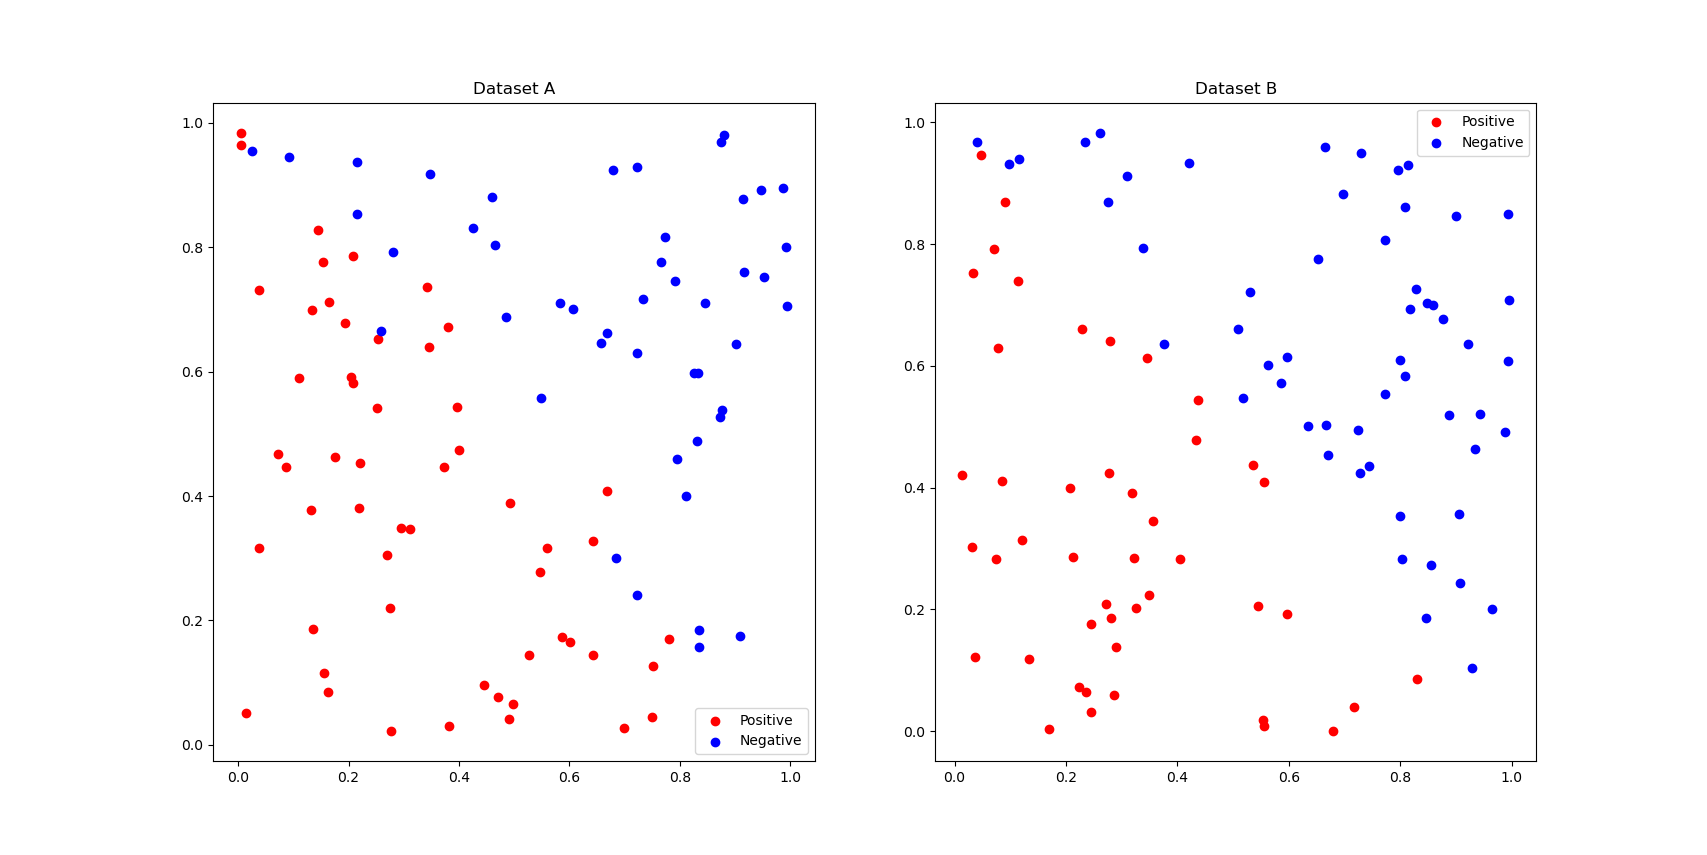
\includegraphics[width=0.7\linewidth]{01-stability/assets/datasets}
		\caption{}
		\label{fig:datasets}
	\end{figure}
	
	By observing the code, we find the gradient of loss function $J(\theta)$ is
	
	$$
	\nabla_{\theta} J(\theta) = -\frac{1}{m}\sum_{i = 1}^m \frac{x^{(i)}y^{(i)}}{1 + \exp(y^{(i)} \theta^T x^{(i)})}\\
	$$
	
	So we can infer what $J(\theta)$ is:
	
	$$
	J(\theta) = -\frac{1}{m}\sum_{i=1}^{m} \ln\frac{1}{1 + \exp(-y^{(i)} \theta^T x^{(i)})}
	$$
	
	For dataset $B$, which is linear separable, all examples within $B$ satisfies $y^{(i)}\theta^T x^{(i)}>0$, while there exists some examples within $A$ that satisfies $y^{(i)}\theta^T x^{(i)}<0$, since $A$ is not linear separable.
	
	For those examples $(x^{(i)}, y^{(i)})$ in $A$ that can't be classified correctly with a certain $\theta$, adjusting $\theta$ to make those examples well classified requires breaking the current situation where the hypothesis performs well on most examples and making $J(\theta)$ bigger. So the algorithm will leave $J(\theta)$ approximately unchanged by returning a gradient of a small norm, in other words, $J(\theta)$ converges.
	
	In contrast, there always exists a way to decrease $J(\theta)$ of dataset $B$, so $J(\theta)$ will keep decreasing rather than converge until it is truly very closed to the minimum.
\end{answer}
